\section{Appendix}
\label{sec:appendix}
\subsection{Configurations of devices}
% \subsection{Controlling the setup with the oscilloscope}
\begin{table}[H]
    \centering
    \begin{tabular}{|l|l|}
        \hline
        coarse grain    & 200\\
        gain            &   10.0 \\
        sharpening time &   0.5 $\mu$s\\
        sample          & position 1\\
        detector        & right \\
        output          & to unipolar MCA\\
        BLR             & "AFJ" \\
        +/-             & "Pos" \\
        delay           & "out" \\
        \hline
    \end{tabular}
    \label{tab:config}
    \caption{
        Configuration of the MA for measurement of the energy spectrum.
        }
\end{table}

% \subsubsection{Measuring the full energy spectrum}
\begin{table}[htp]
    \centering
    \begin{tabular}{|l|l|l||l|l|l|}
        \hline
        2.1a) & position  & Pos1         & 2.1b) & position  & Pos1\\
              & detector          & right        &       & detector          & left \\
              & time        & $360\pm1$sec &       & time        & $380\pm1$sec \\
        \hline 
        2.1c) & position  & Pos2         & 2.1d) & position  & Pos2         \\
              & detector          & right        &       & detector          & left \\
              & time        & $402\pm1$sec &       & time        & $368\pm1$sec \\
        \hline 
        2.1e) & position  & Pos2         \\
              & detector          & left \\
              & time        & $360\pm1$sec \\
    \cline{1-3}
    \end{tabular}
    \caption{
        Configurations in measurement of energy spectrum of $^{57}$Co.
        "Pos1" and "Pos2" are defined as shown in figure \ref{fig:position_1}. 
        "time" is referring to the time over which the spectrum was recorded. 
        The results are shown in figures \ref{fig:measure2.1}.
        }
    \label{tab:config2}
\end{table}
\clearpage

\subsection{Additional figures}
\subsubsection{Energy spectrum of $^{57}$Co}
\begin{figure}[H]
    \begin{subfigure}[b]{\picwidth}
        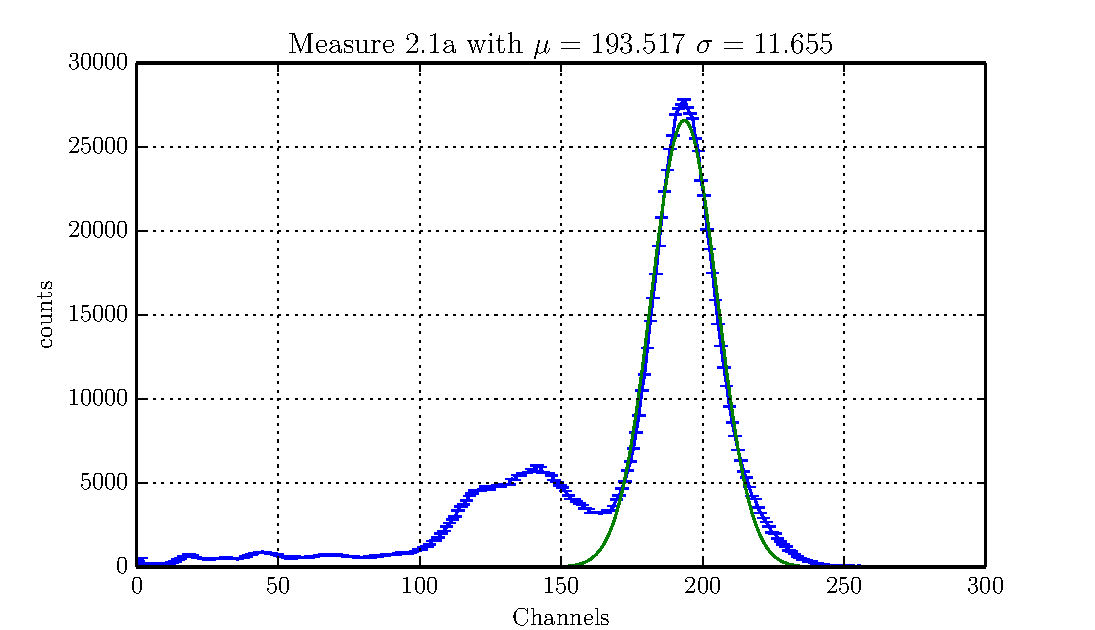
\includegraphics[width=\textwidth]{analysis/figures/plot2_1a}
        \caption{}
    \end{subfigure}\qquad
    \begin{subfigure}[b]{\picwidth}
        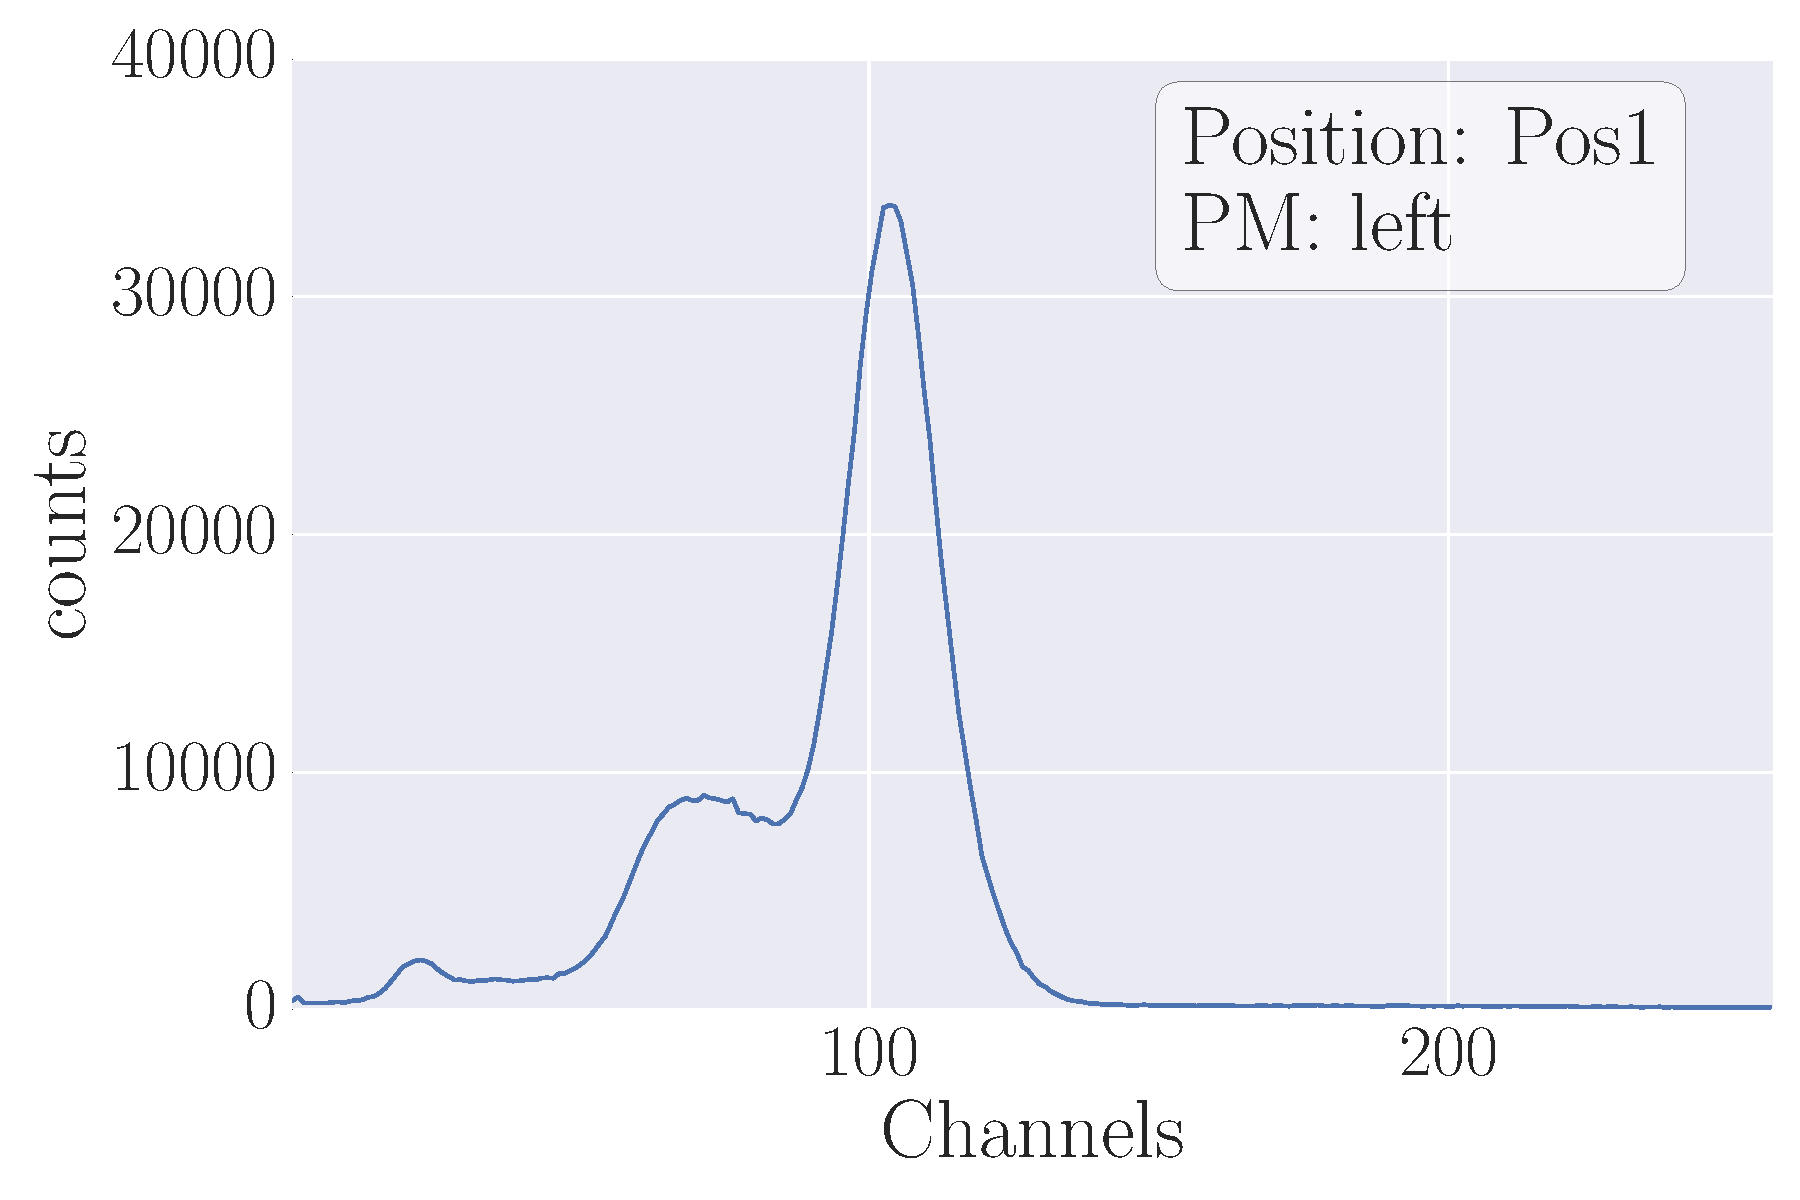
\includegraphics[width=\textwidth]{analysis/figures/plot2_1b}
        \caption{}
    \end{subfigure}
    \begin{subfigure}[b]{\picwidth}
        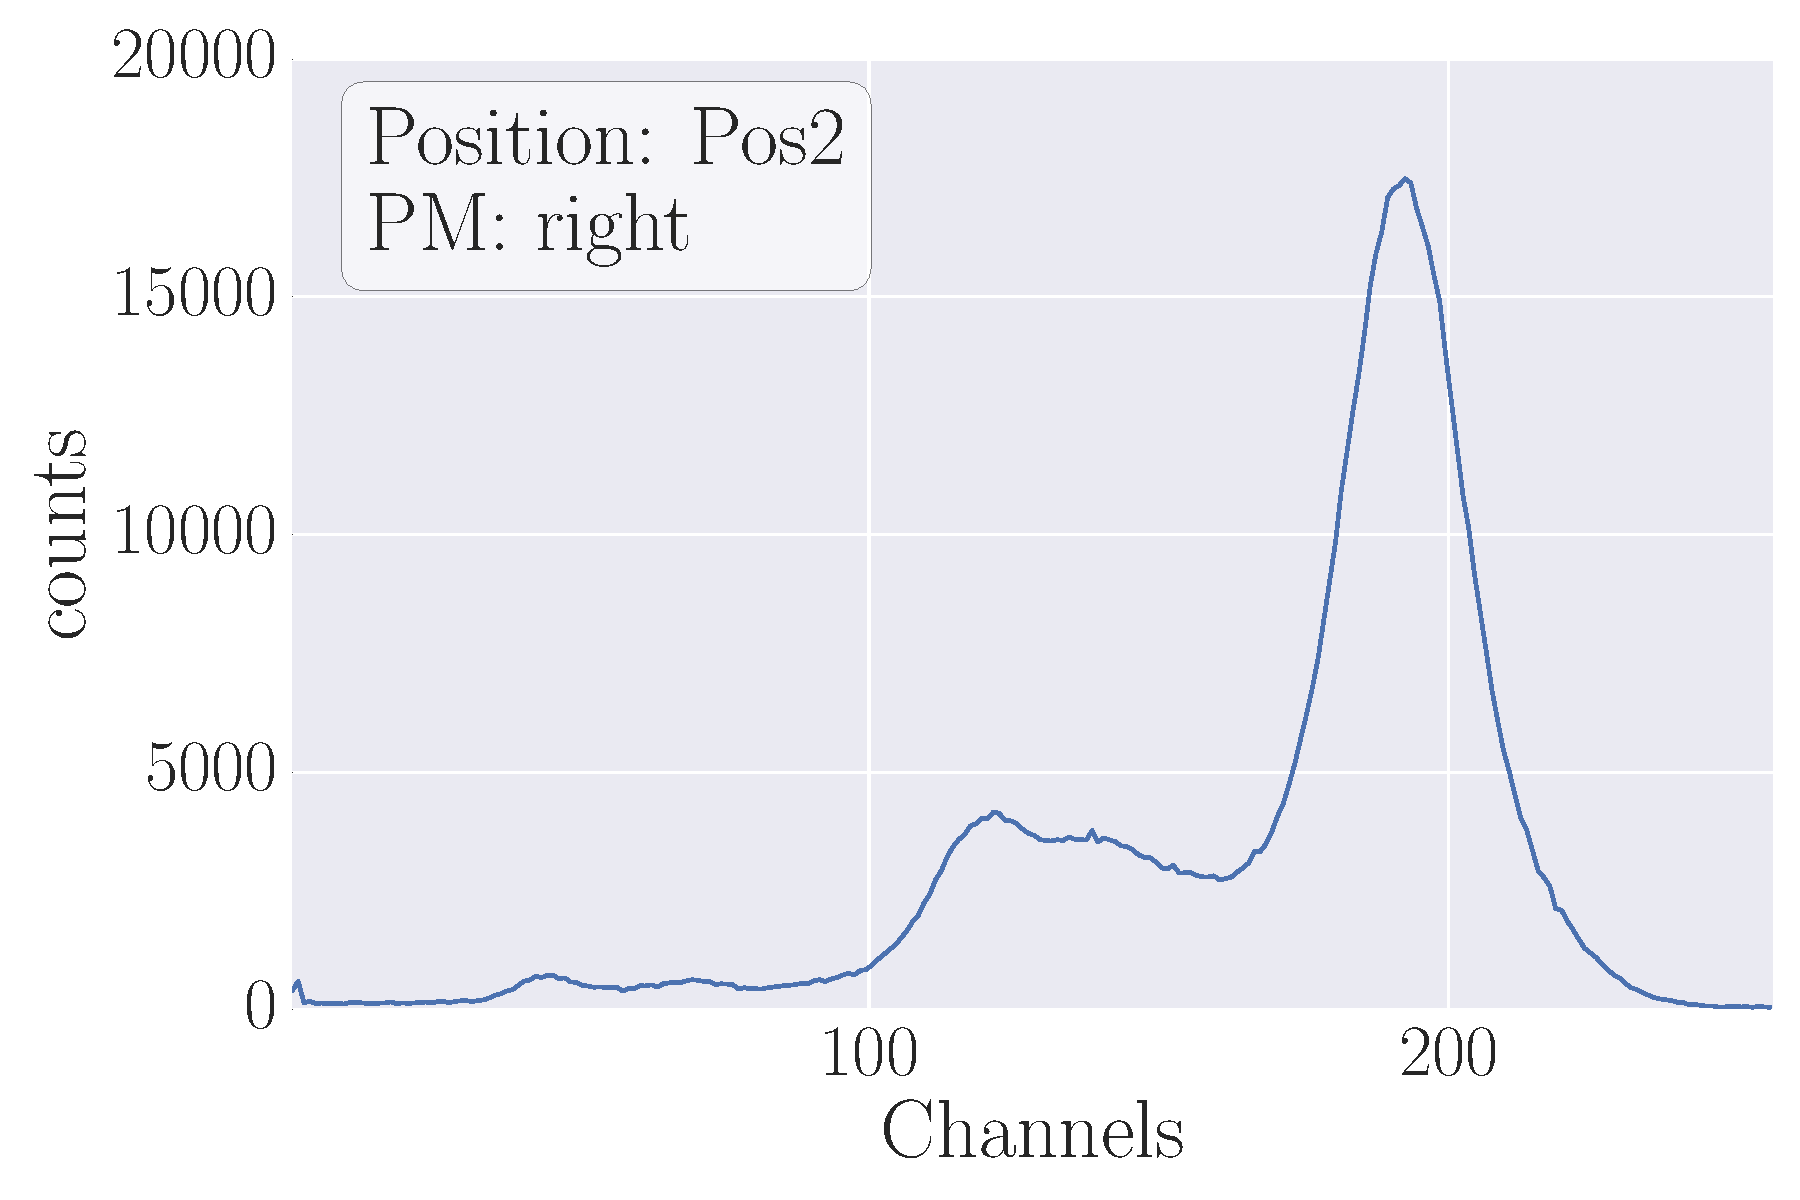
\includegraphics[width=\textwidth]{analysis/figures/plot2_1c}
        \caption{}
    \end{subfigure}
    \begin{subfigure}[b]{\picwidth}
        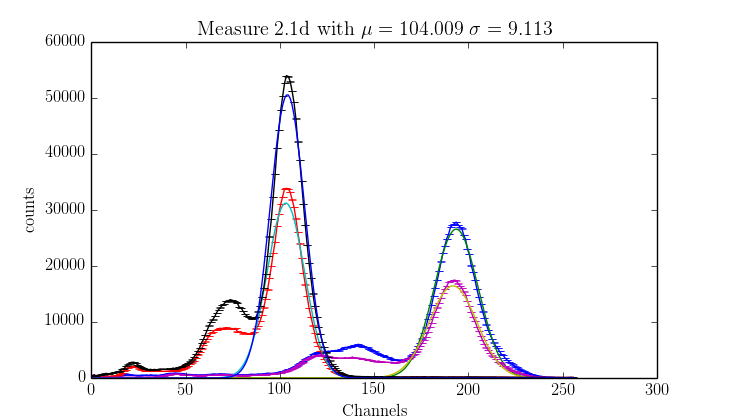
\includegraphics[width=\textwidth]{analysis/figures/plot2_1d}
        \caption{}
    \end{subfigure}
    \begin{subfigure}[b]{\picwidth}
        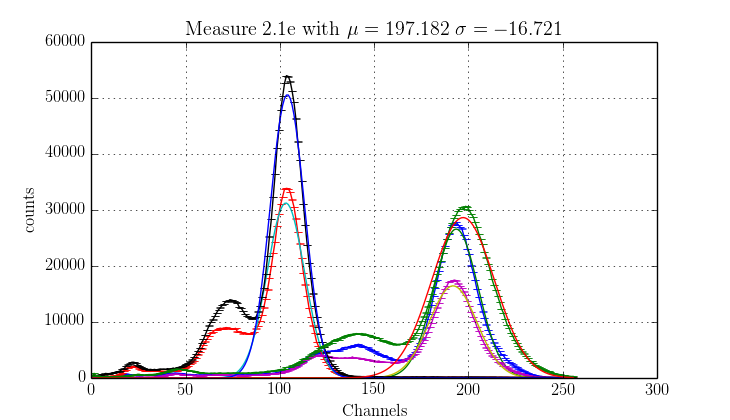
\includegraphics[width=\textwidth]{analysis/figures/plot2_1e}
        \caption{}
    \end{subfigure}
    \caption{
        Histograms of events recorded with the MCA, thus corresponding to the energy 
        spectrum of the probe. Each histogram corresponds to a combination of position 
        of the probe and used detector, as classified in table \ref{tab:config2}
        }
    \label{fig:measure2.1}
\end{figure}

\subsubsection{Energy spectrum of $^{241}$Am}
\begin{figure}[H]
    \centering
    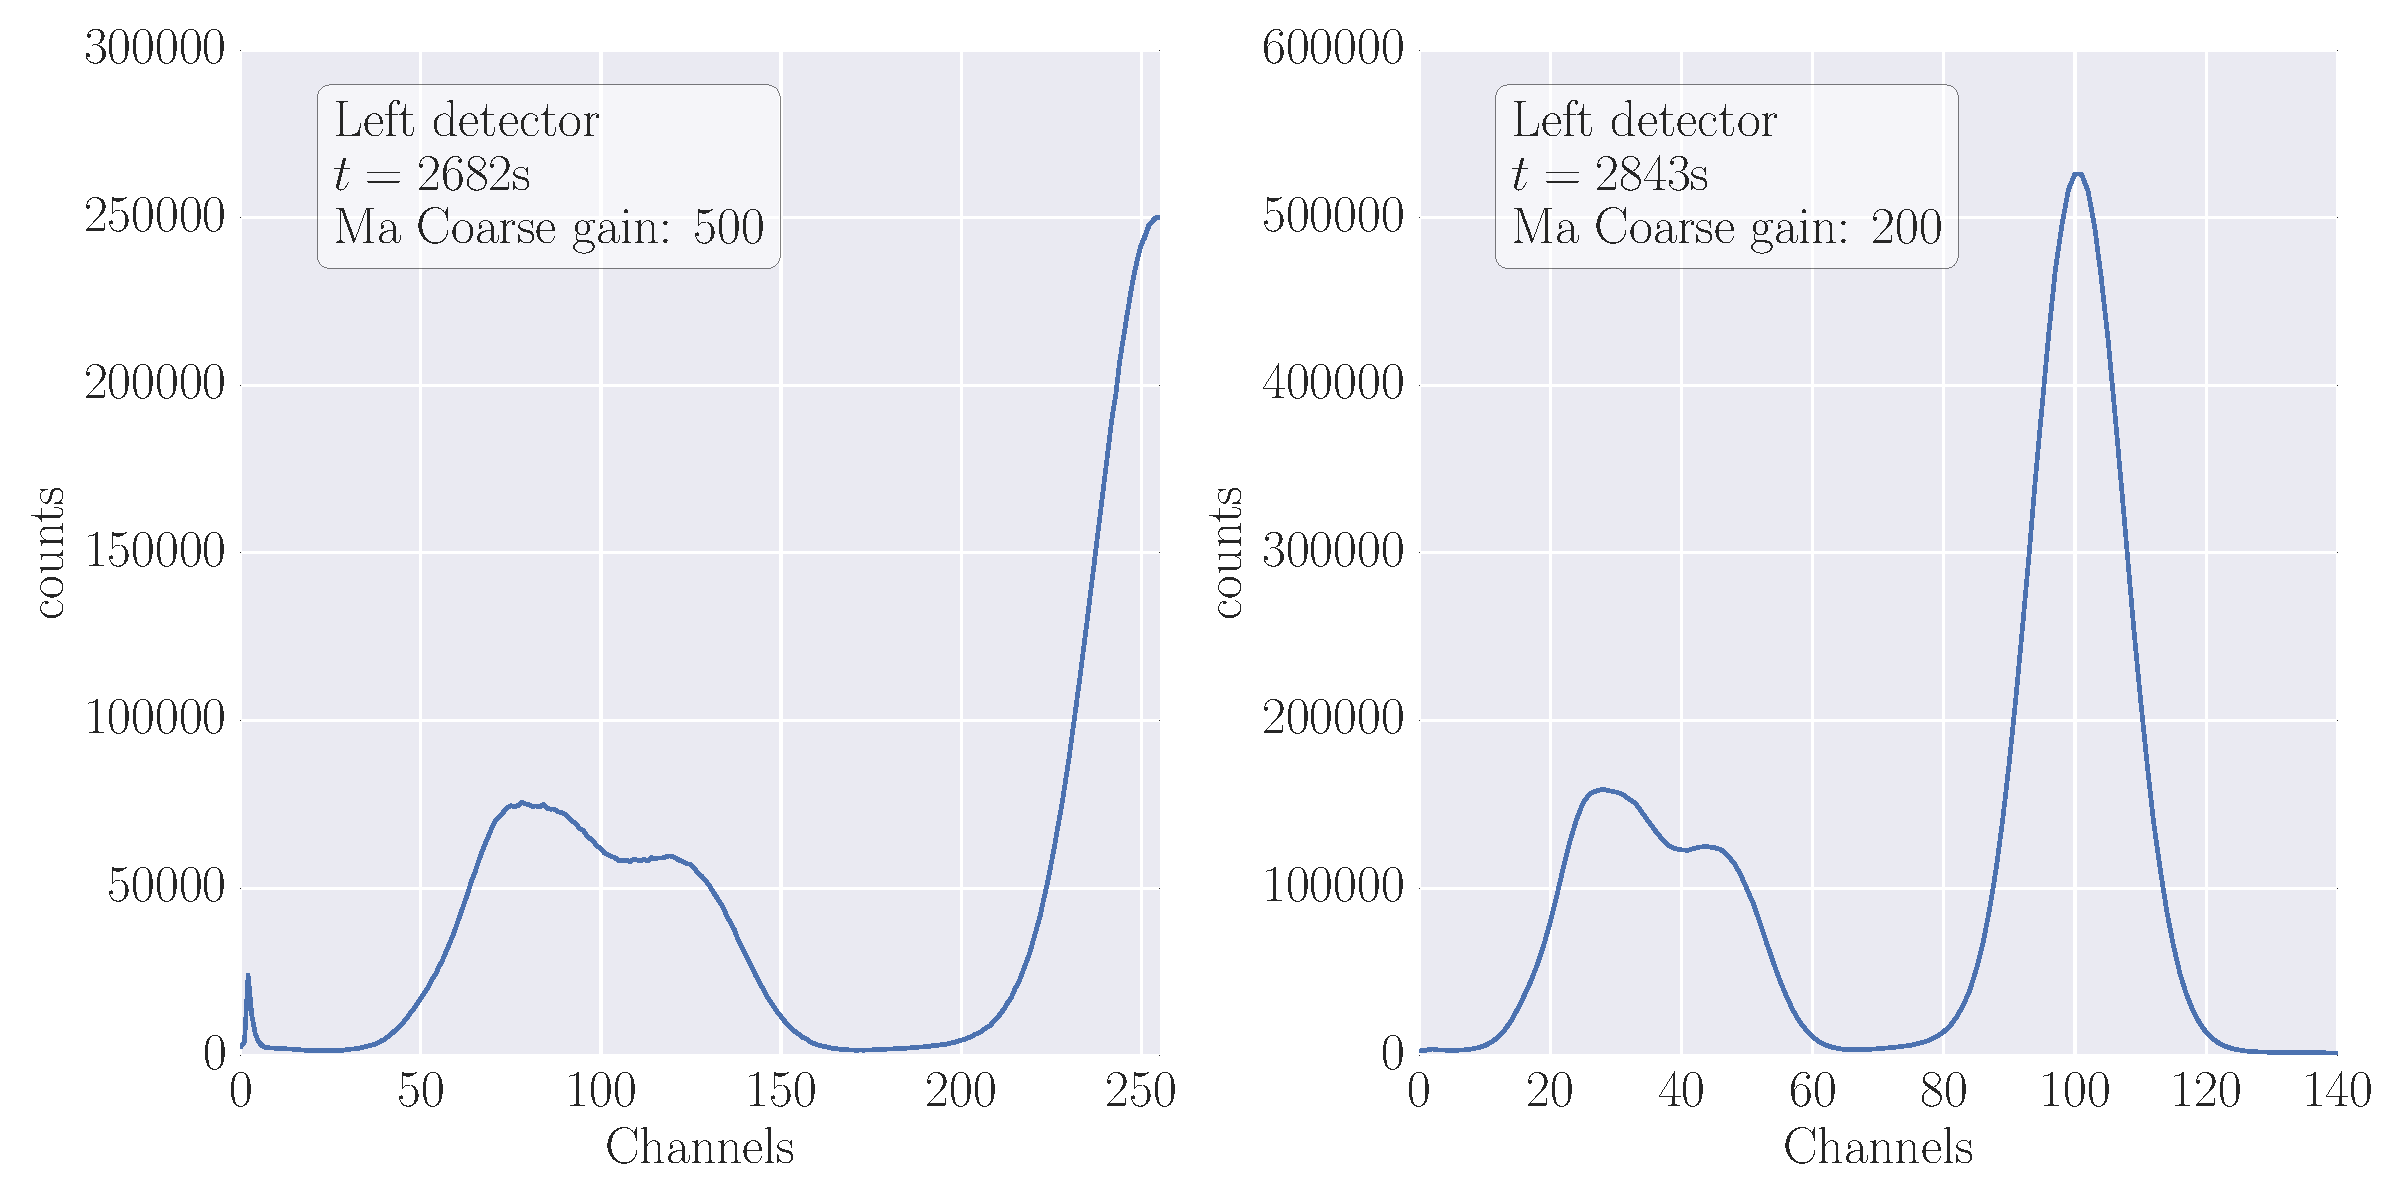
\includegraphics[width=\linewidth]{analysis/figures/plot6_12}
    \caption{$^{241}Am$ energy spectrum}
    \label{fig:plot6_13}
\end{figure}
\begin{figure}[H]
    \centering
    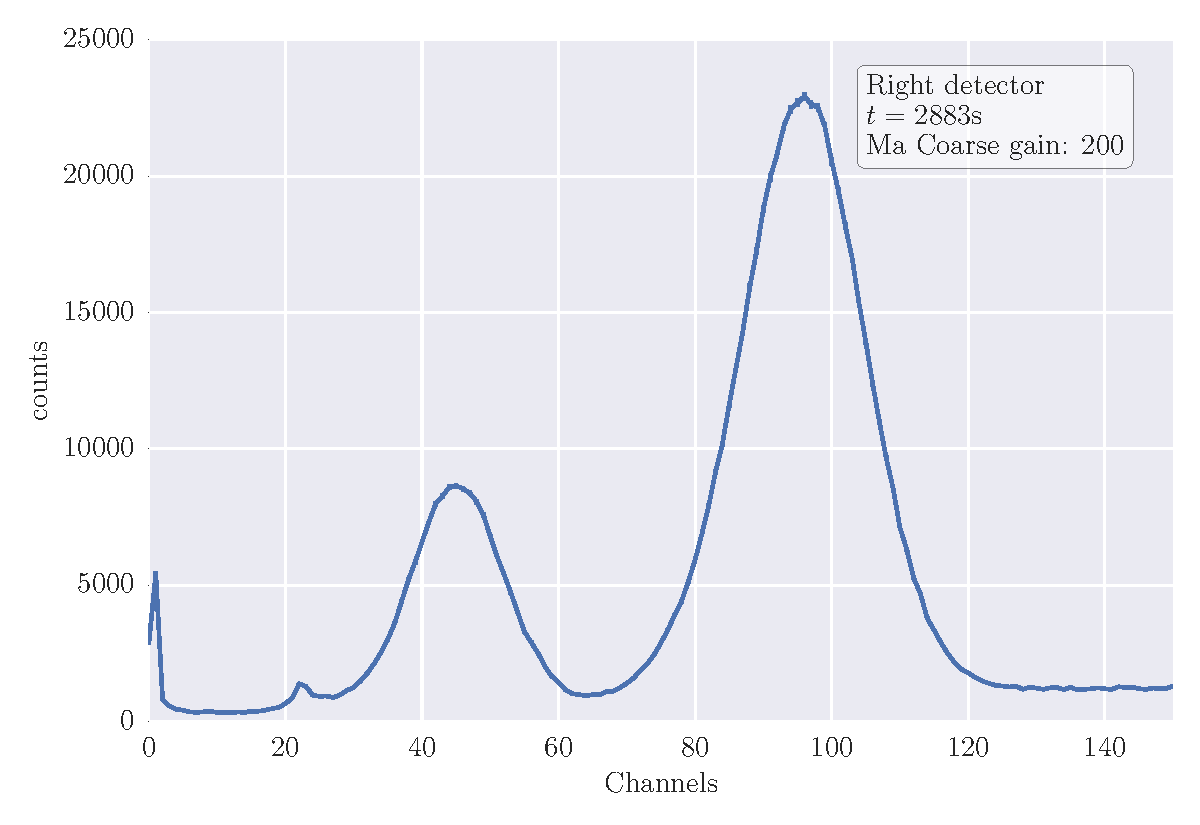
\includegraphics[width=0.8\linewidth]{analysis/figures/plot6_3}
    \caption{$^{241}Am$ energy spectrum}
    \label{fig:plot6_13}
\end{figure}
\clearpage

\subsection{Covariance matrices}
\subsubsection{Covariance matrix of $^{57}$Co energy spectrum}
\label{subs:covariance}
This is the covariance matrix and the parameters for the cobalt probe, see
figure~\ref{fig:fit1} for the figure.
   \begin{align*}
    A_1 &=& \left(3.6 \pm 1.2\right) \times 10^{2} \quad \mathrm{counts}\\
    A_2 &=& \left(5.7 \pm 0.4\right) \times 10^{2} \quad \mathrm{counts}\\
    A_3 &=& \left(1.11 \pm 0.28\right) \times 10^{3} \quad \mathrm{counts}\\
    A_4 &=& \left(5.55 \pm 0.14\right) \times 10^{3} \quad \mathrm{counts}\\
    A_5 &=& \left(2.555 \pm 0.030\right) \times 10^{4} \quad \mathrm{counts}\\
    \mu_1 &=& 18.2 \pm 0.8 \quad \mathrm{channels}\\
    \mu_2 &=& 61.6 \pm 4.1 \quad \mathrm{channels}\\
    \mu_3 &=& 115.8 \pm 1.2 \quad \mathrm{channels}\\
    \mu_4 &=& 138.0 \pm 0.9 \quad \mathrm{channels}\\
    \mu_5 &=& 193.76 \pm 0.13 \quad \mathrm{channels}\\ \sigma_1 &=& 1.7 \pm 0.6 \quad \mathrm{channels}\\ \sigma_2 &=& 22.8 \pm 2.9 \quad \mathrm{channels}\\ \sigma_3 &=& 4.0 \pm 1.1 \quad \mathrm{channels}\\
    \sigma_4 &=& 12.8 \pm 0.5 \quad \mathrm{channels}\\
    \sigma_5 &=& 8.33 \pm 0.08 \quad \mathrm{channels}\\
    c &=& 124.6 \pm 16.5 counts
    \end{align*}
\tiny
\begin{equation*}
    \begin{pmatrix}
        14246.0 &48.6 &-285.5 &159.0 &7.3 &-2.2 &13.0 &-0.5 &-1.5 &0.0 &-35.1 &-27.2 &-0.7 &0.9 &-0.0 &26.7 \\
        48.6 &1346.9 &673.0 &446.5 &-26.3 &-1.5 &-9.5 &-0.7 &1.4 &-0.0 &0.8 &-26.9 &3.0 &-1.2 &0.2 &-243.2 \\
        -285.5 &673.0 &79641.9 &-12911.5 &823.7 &6.7 &587.9 &51.1 &178.2 &-3.5 &-4.7 &334.8 &112.3 &-88.5 &1.8 &-173.2 \\
        159.0 &446.5 &-12911.5 &20593.7 &-478.5 &-1.8 &-98.5 &-72.3 &-54.0 &-1.7 &2.4 &-68.5 &-62.3 &-6.1 &1.1 &-169.3 \\
        7.3 &-26.3 &823.7 &-478.5 &91725.2 &-0.1 &-12.6 &8.0 &14.6 &1.4 &0.1 &-7.6 &3.5 &6.9 &-14.0 &14.4 \\
        -2.2 &-1.5 &6.7 &-1.8 &-0.1 &0.7 &0.2 &0.0 &0.0 &-0.0 &0.0 &0.2 &0.0 &-0.0 &0.0 &0.1 \\
        13.0 &-9.5 &587.9 &-98.5 &-12.6 &0.2 &17.2 &0.5 &2.3 &-0.1 &0.1 &8.3 &1.9 &-1.6 &0.1 &-1.7 \\
        -0.5 &-0.7 &51.1 &-72.3 &8.0 &0.0 &0.5 &1.4 &0.3 &0.0 &-0.0 &0.3 &0.4 &0.0 &-0.0 &-0.1 \\
        -1.5 &1.4 &178.2 &-54.0 &14.6 &0.0 &2.3 &0.3 &0.8 &0.0 &-0.0 &1.4 &0.7 &-0.3 &-0.0 &-0.9 \\
        0.0 &-0.0 &-3.5 &-1.7 &1.4 &-0.0 &-0.1 &0.0 &0.0 &0.0 &0.0 &-0.1 &-0.0 &0.0 &-0.0 &-0.0 \\
        -35.1 &0.8 &-4.7 &2.4 &0.1 &0.0 &0.1 &-0.0 &-0.0 &0.0 &0.4 &-0.4 &-0.0 &0.0 &-0.0 &0.2 \\
        -27.2 &-26.9 &334.8 &-68.5 &-7.6 &0.2 &8.3 &0.3 &1.4 &-0.1 &-0.4 &8.2 &1.0 &-0.9 &0.0 &-12.4 \\
        -0.7 &3.0 &112.3 &-62.3 &3.5 &0.0 &1.9 &0.4 &0.7 &-0.0 &-0.0 &1.0 &1.3 &-0.3 &0.0 &-0.5 \\
        0.9 &-1.2 &-88.5 &-6.1 &6.9 &-0.0 &-1.6 &0.0 &-0.3 &0.0 &0.0 &-0.9 &-0.3 &0.3 &-0.0 &0.4 \\
        -0.0 &0.2 &1.8 &1.1 &-14.0 &0.0 &0.1 &-0.0 &-0.0 &-0.0 &-0.0 &0.0 &0.0 &-0.0 &0.0 &-0.2 \\
        26.7 &-243.2 &-173.2 &-169.3 &14.4 &0.1 &-1.7 &-0.1 &-0.9 &-0.0 &0.2 &-12.4 &-0.5 &0.4 &-0.2 &272.5 \\
    \end{pmatrix}
   \end{equation*}
   \normalsize
   \\\\
 \clearpage

\subsubsection{Covariance matrix of $^{241}$Am energy spectrum}
This is the covariance matrix and the parameters for the americium probe, see
figure~\ref{fig:fit2} for the figure.
\begin{align*}
    A_1 &=& \left(6.7 \pm 5.4\right) \times 10^{2} \quad \mathrm{counts}\\
    A_2 &=& \left(7.95 \pm 0.29\right) \times 10^{3} \quad\mathrm{counts}\\
    A_3 &=& \left(2.16 \pm 0.04\right) \times 10^{4} \quad\mathrm{counts}\\
    \mu_1 &=& 22.4 \pm 0.4 \quad\mathrm{channels}\\
    \mu_2 &=& 45.24 \pm 0.21 \quad\mathrm{channels}\\
    \mu_3 &=& 95.74 \pm 0.14 \quad\mathrm{channels}\\
    \sigma_1 &=& -0.4 \pm 0.4 \quad\mathrm{channels}\\
    \sigma_2 &=& 4.54 \pm 0.13 \quad\mathrm{channels}\\
    \sigma_3 &=& 6.61 \pm 0.08 \quad\mathrm{channels}\\
    c &=& 827.0 \pm 21.6\quad \mathrm{counts}
\end{align*}
\small
\begin{equation*}
    \begin{pmatrix}
        293967.4 &-413.3 &19.7 &28.9 &-0.2 &0.0 &182.9 &0.1 &-0.1 &183.6 \\
        -413.3 &83707.4 &-584.9 &0.3 &-0.4 &-0.2 &-1.7 &-21.7 &0.3 &-119.3 \\
        19.7 &-584.9 &143132.2 &0.0 &0.5 &0.3 &0.1 &0.5 &-18.4 &27.7 \\
        28.9 &0.3 &0.0 &0.2 &0.0 &-0.0 &0.0 &-0.0 &-0.0 &0.1 \\
        -0.2 &-0.4 &0.5 &0.0 &0.0 &0.0 &-0.0 &0.0 &-0.0 &0.0 \\
        0.0 &-0.2 &0.3 &-0.0 &0.0 &0.0 &0.0 &0.0 &-0.0 &0.0 \\
        182.9 &-1.7 &0.1 &0.0 &-0.0 &0.0 &0.2 &0.0 &-0.0 &0.9 \\
        0.1 &-21.7 &0.5 &-0.0 &0.0 &0.0 &0.0 &0.0 &0.0 &-0.5 \\
        -0.1 &0.3 &-18.4 &-0.0 &-0.0 &-0.0 &-0.0 &0.0 &0.0 &-0.3 \\
        183.6 &-119.3 &27.7 &0.1 &0.0 &0.0 &0.9 &-0.5 &-0.3 &467.8 \\
    \end{pmatrix}
\end{equation*}
\normalsize

\subsection{Handwritten records of the experiment}
\label{sec:appendix_records}
    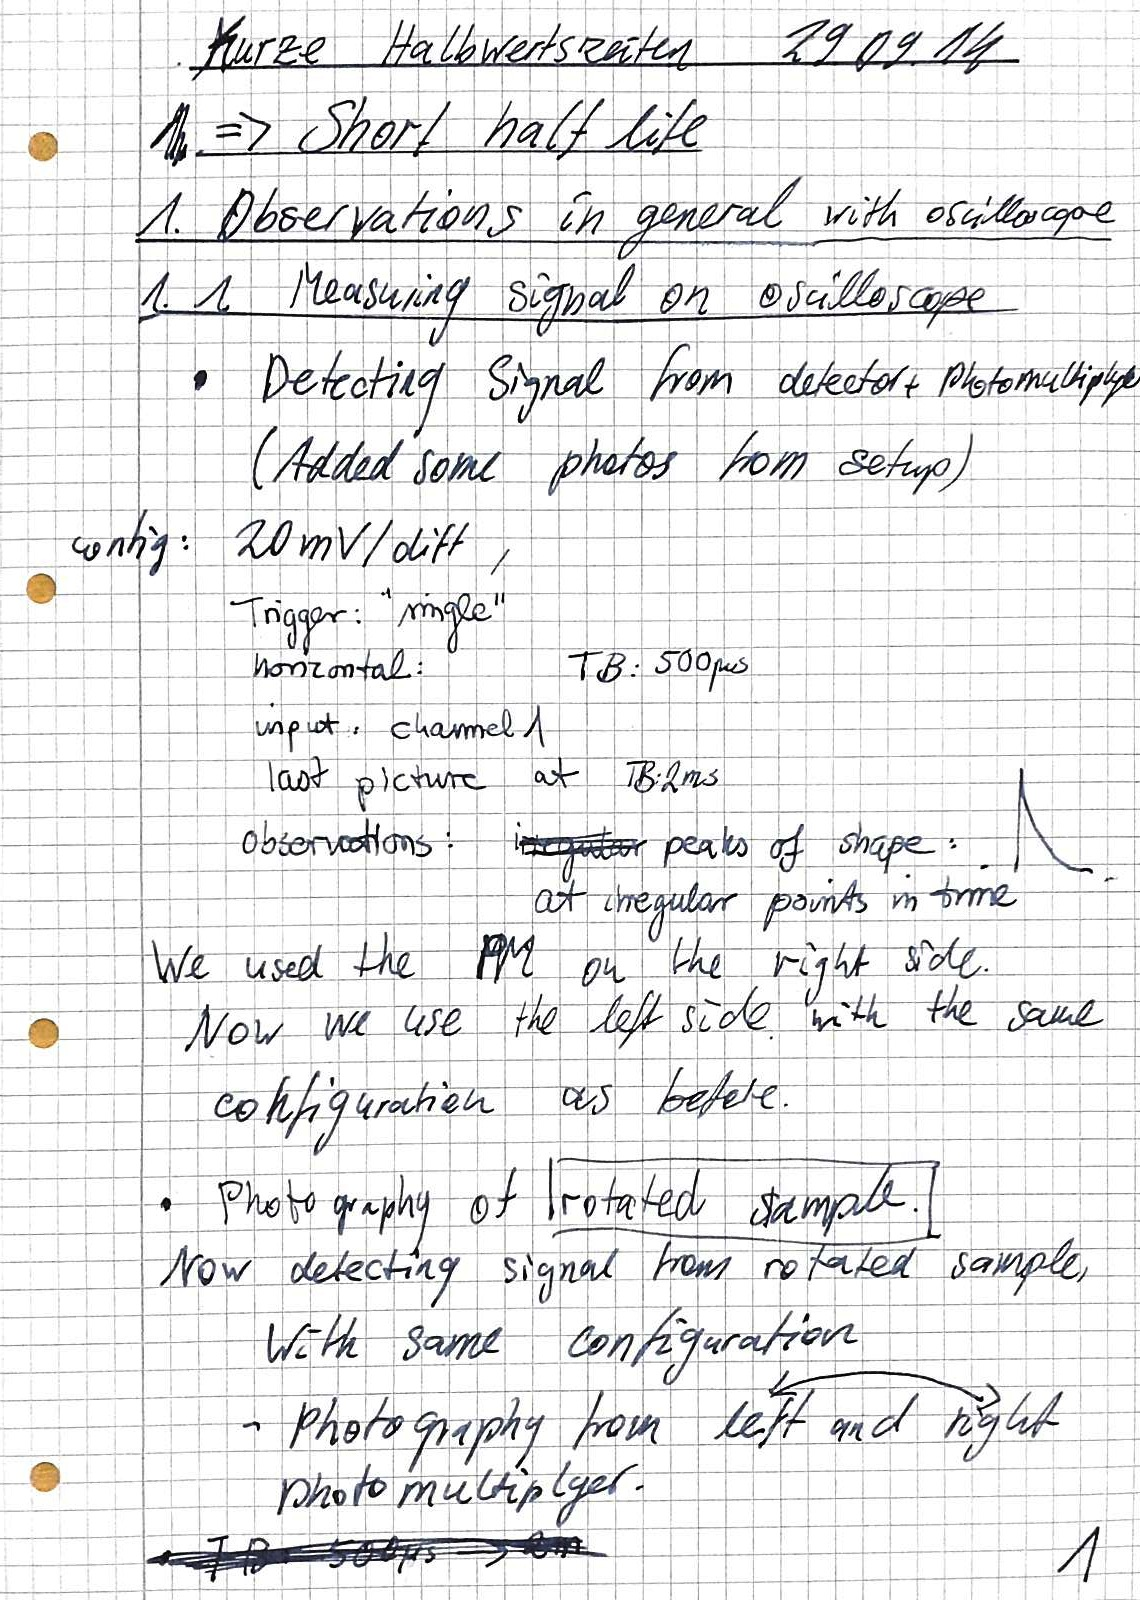
\includegraphics[width=\linewidth]{records/page1.jpeg}
    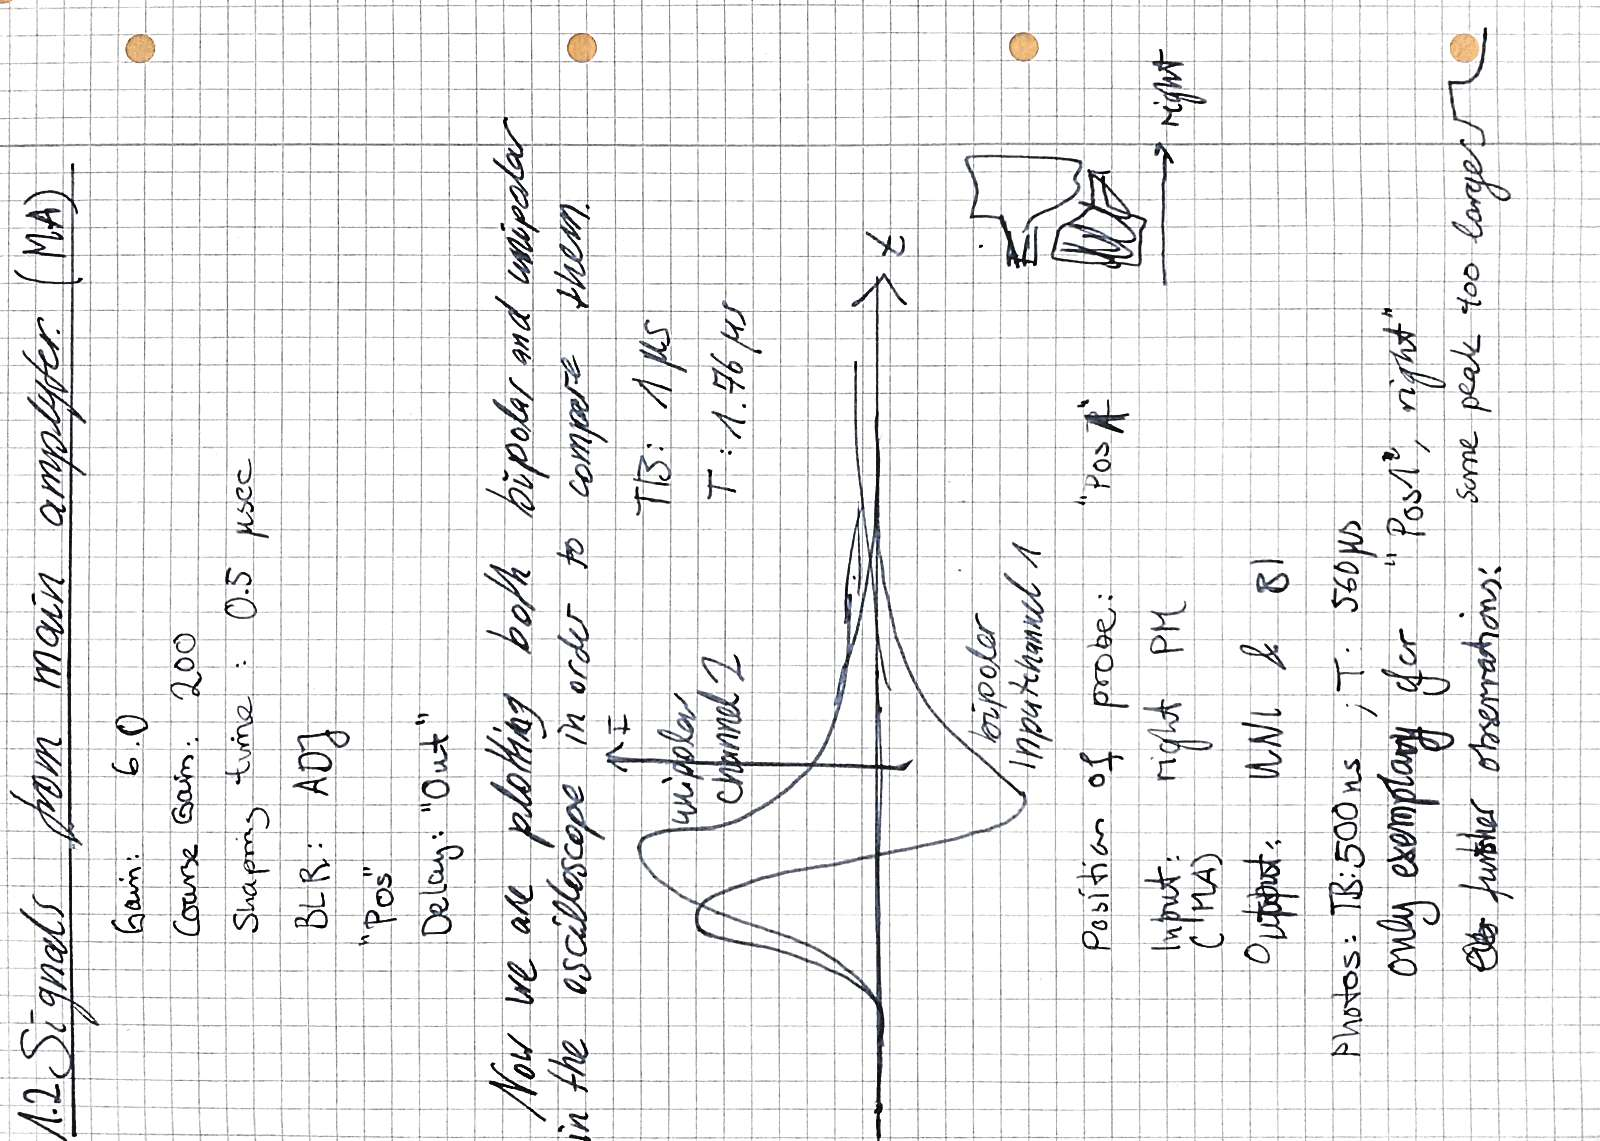
\includegraphics[width=\linewidth]{records/page2.jpeg}
    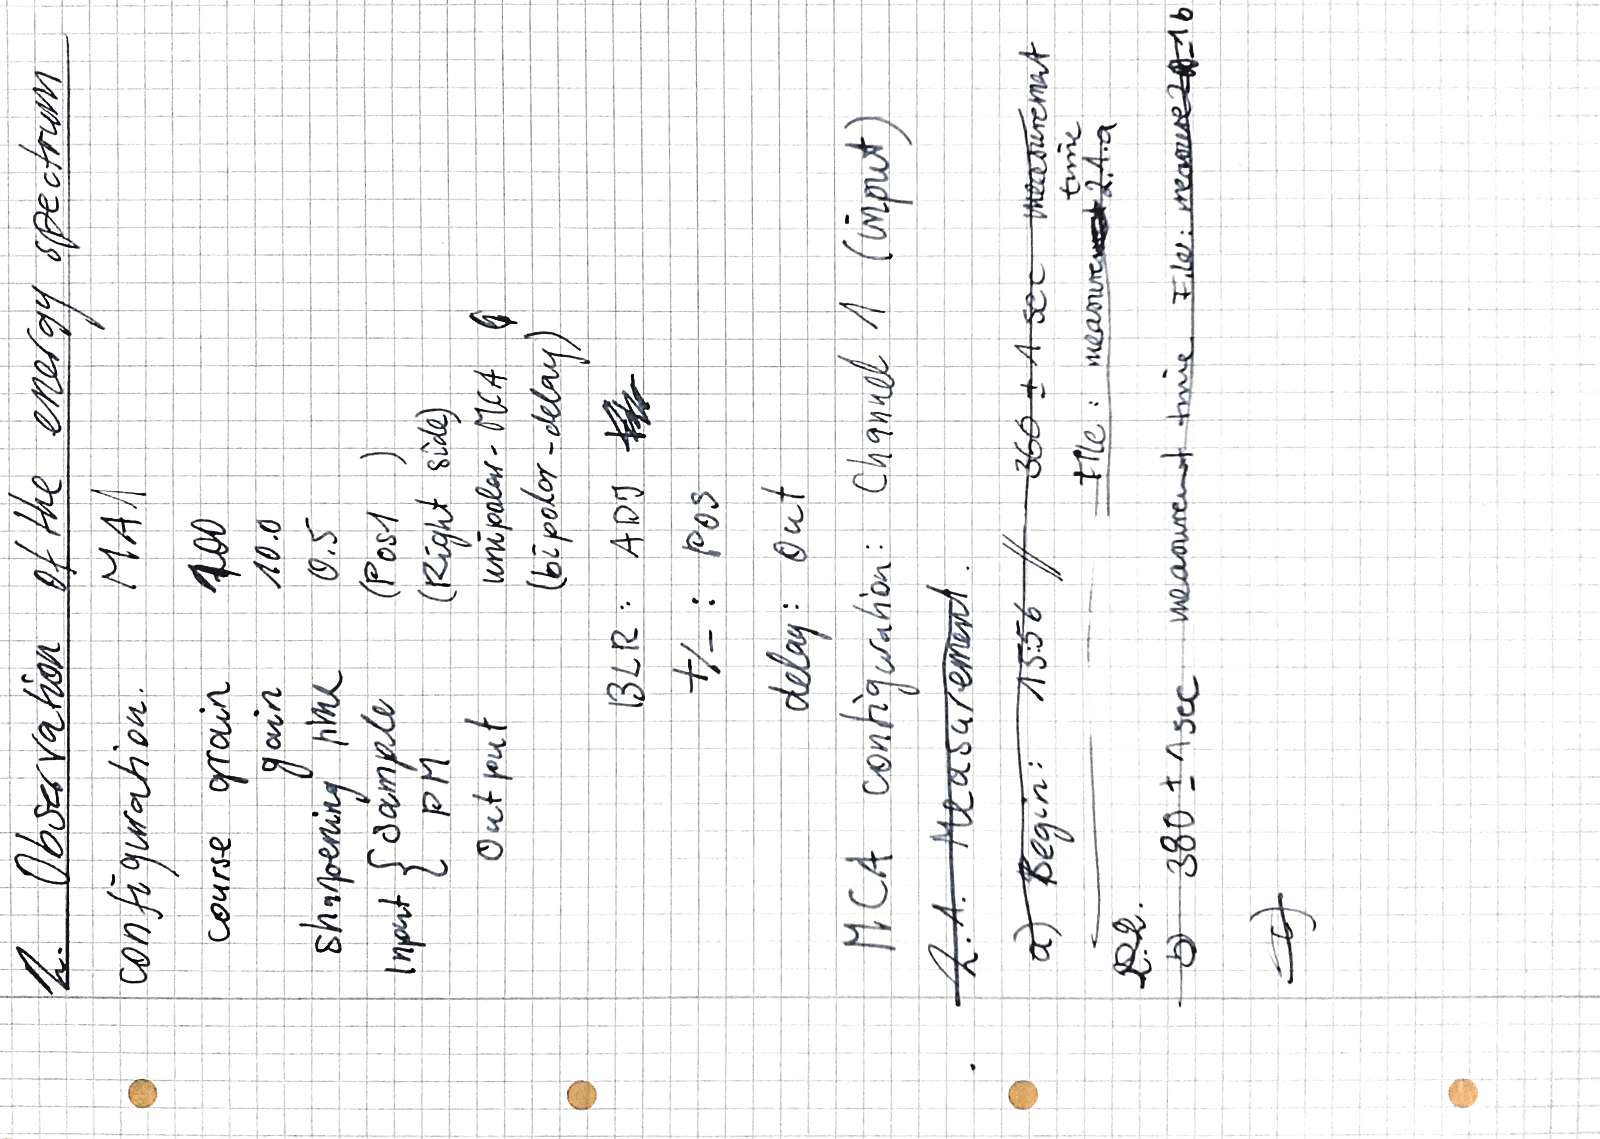
\includegraphics[width=\linewidth]{records/page3.jpeg}
    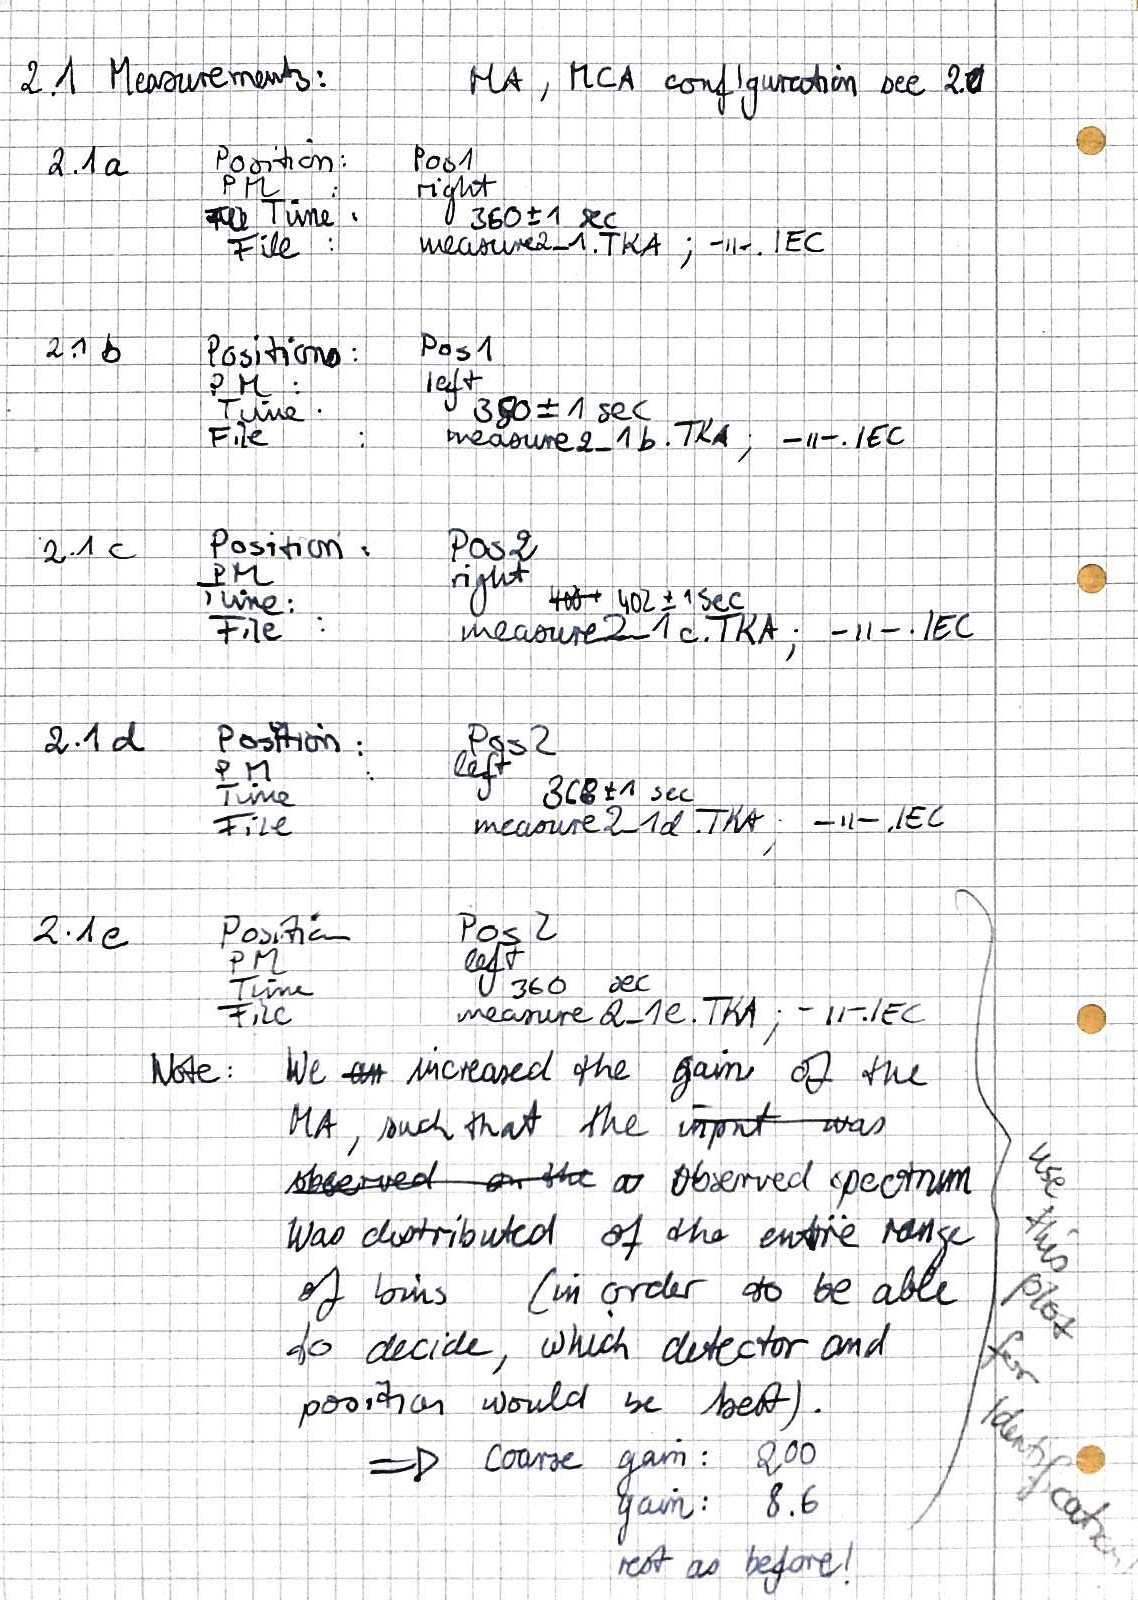
\includegraphics[width=\linewidth]{records/page4.jpeg}
    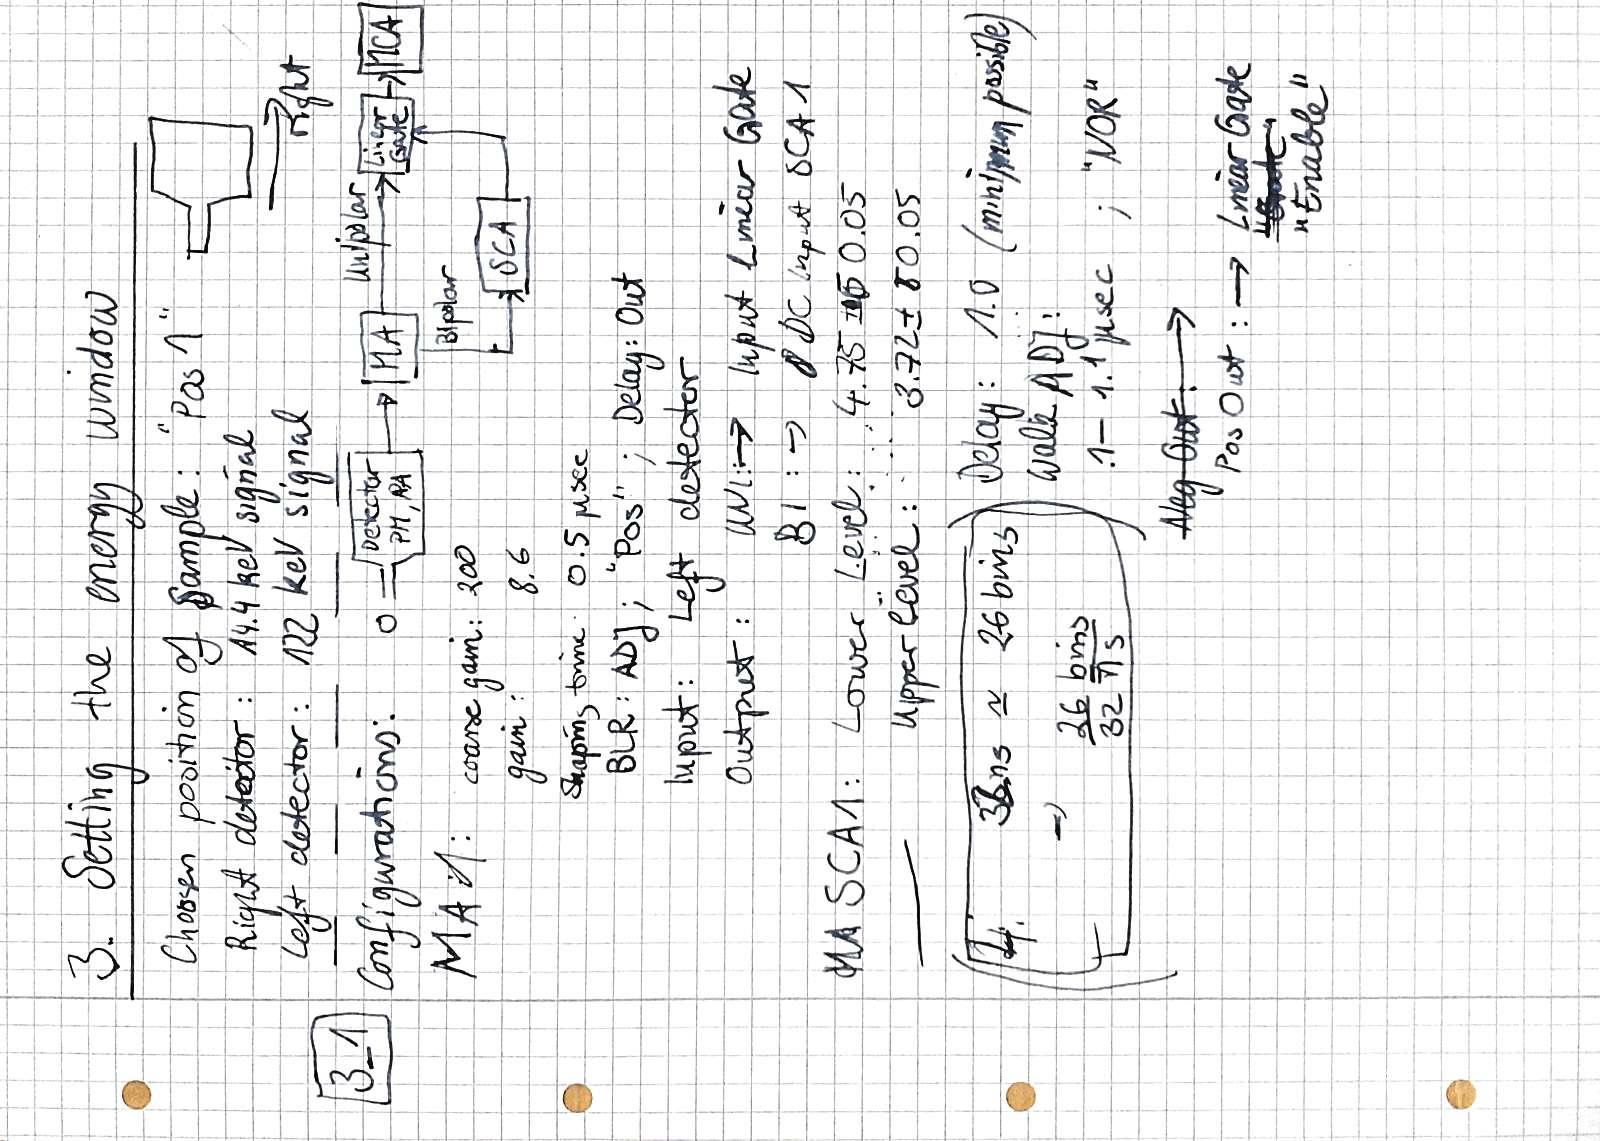
\includegraphics[width=\linewidth]{records/page5.jpeg}
    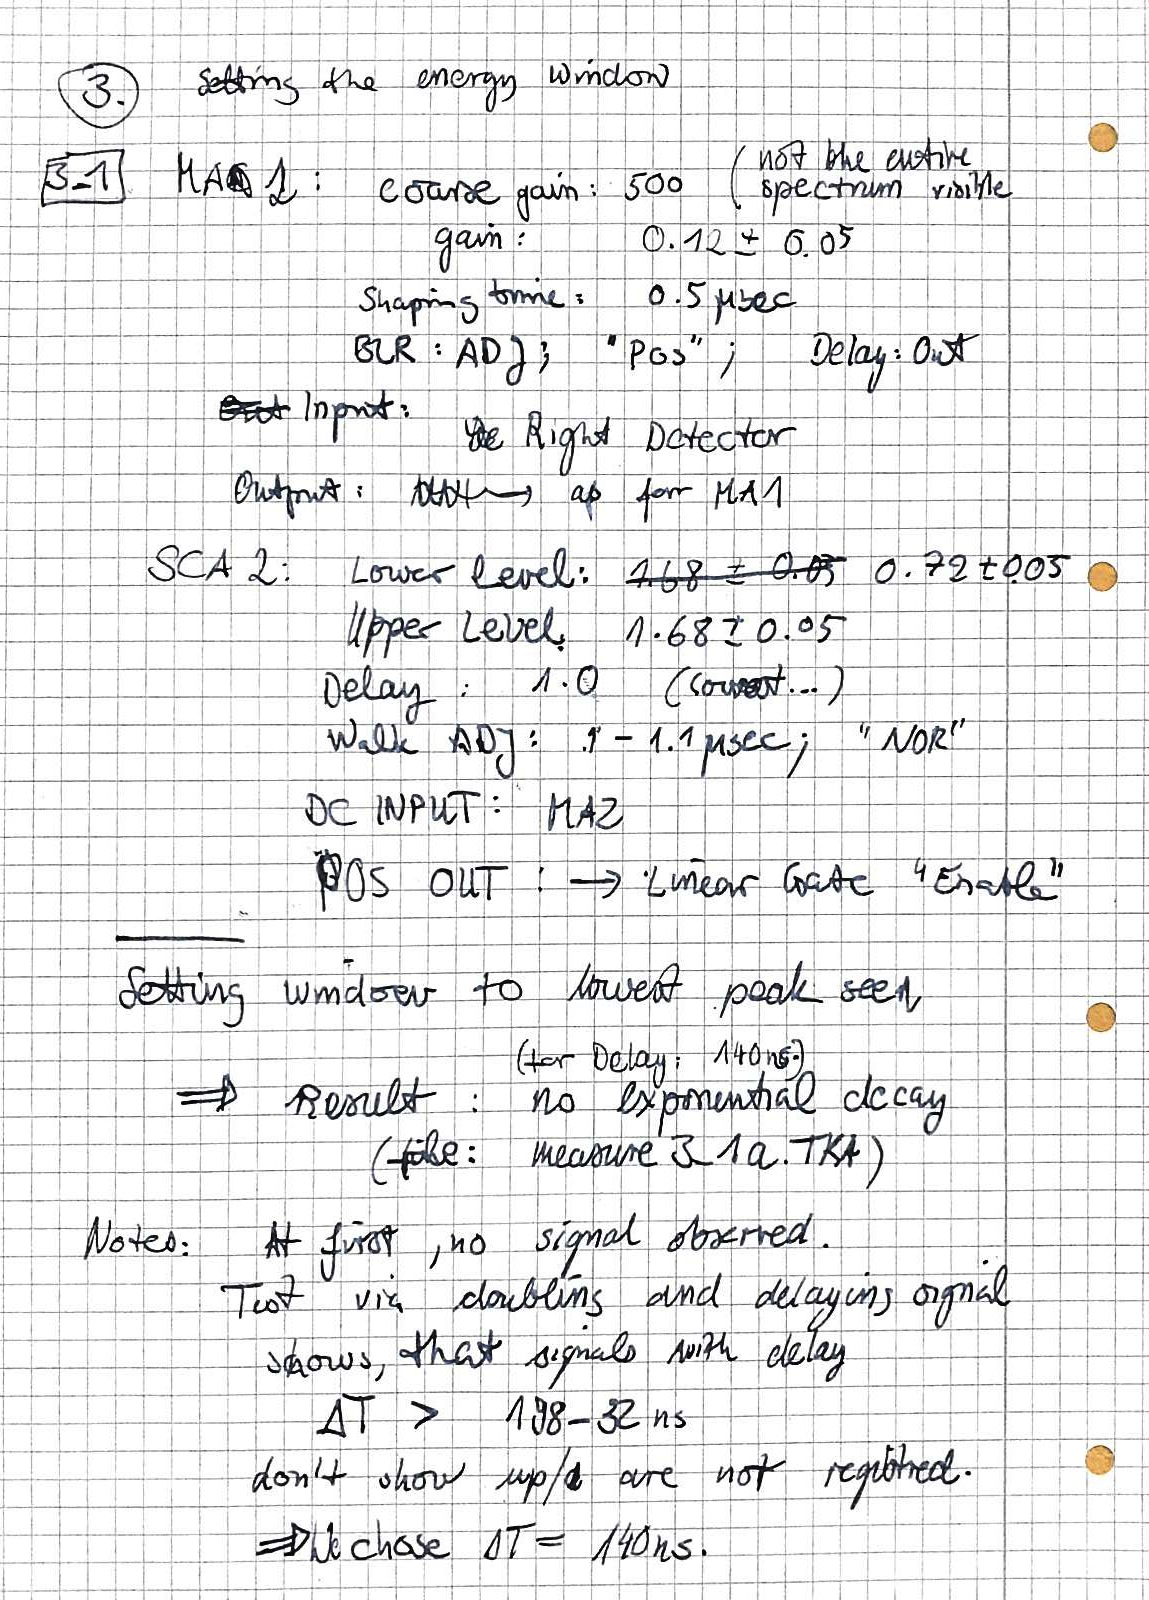
\includegraphics[width=\linewidth]{records/page6.jpeg}
    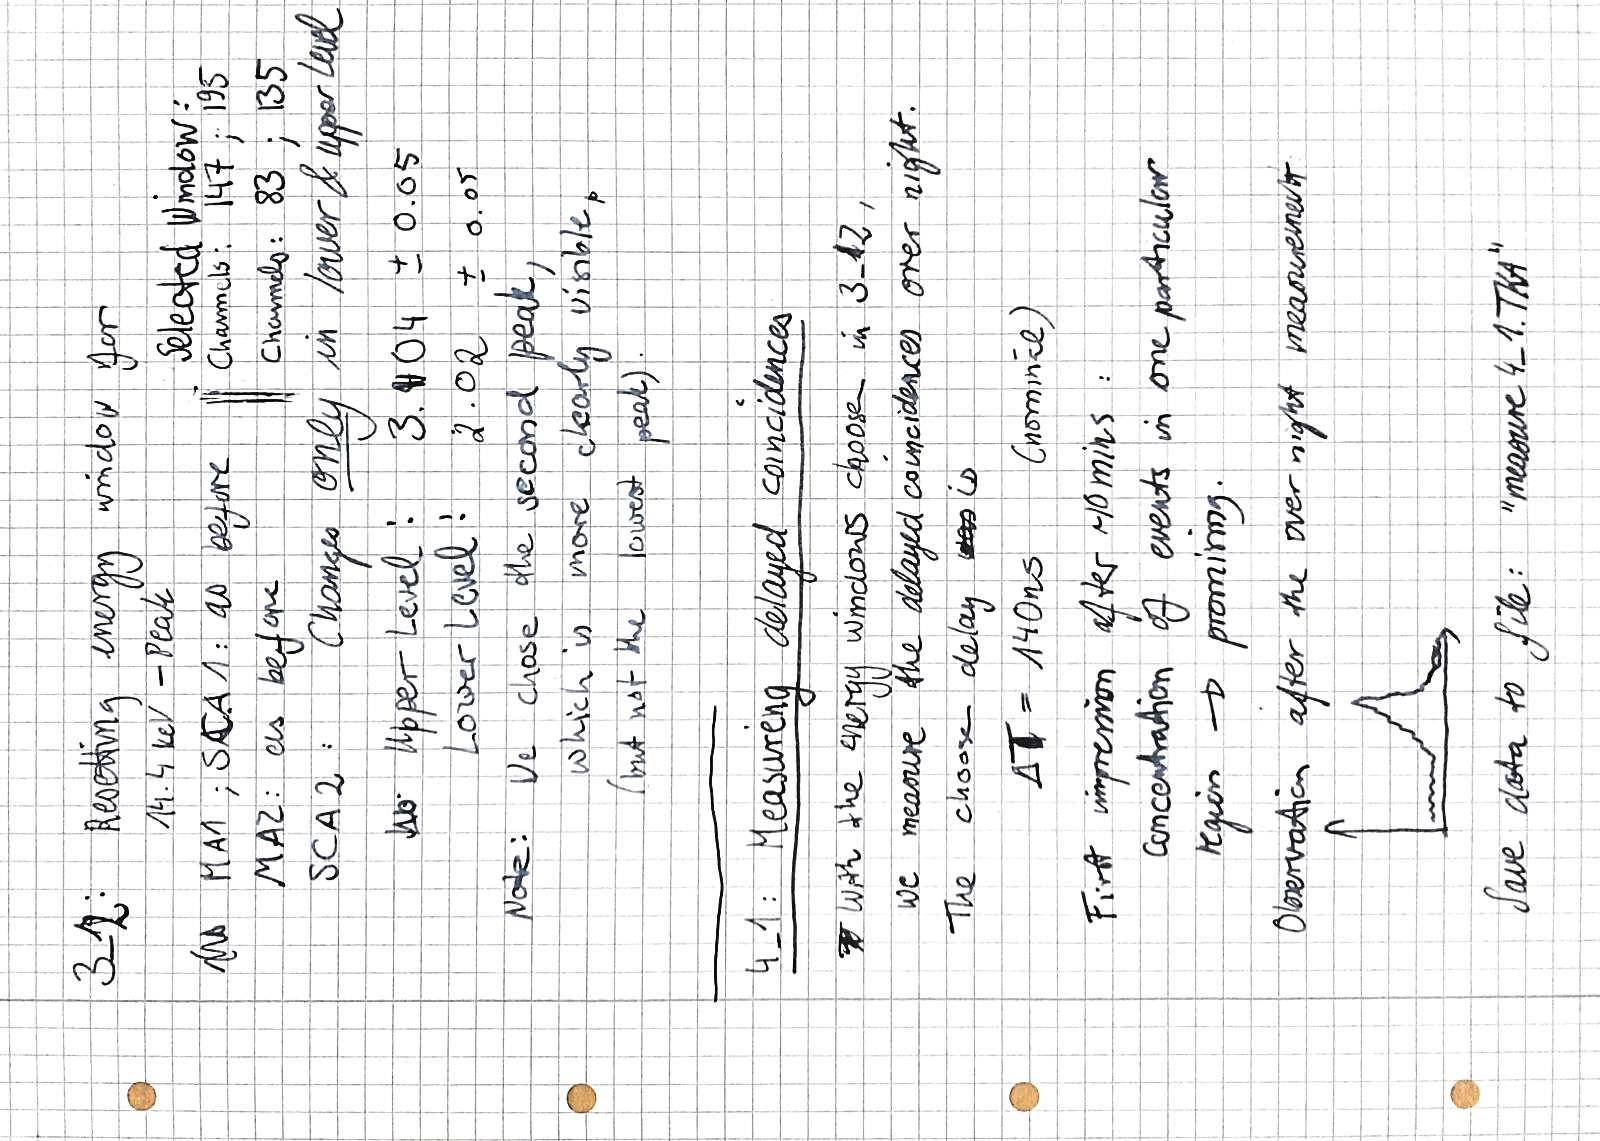
\includegraphics[width=\linewidth]{records/page7.jpeg}
    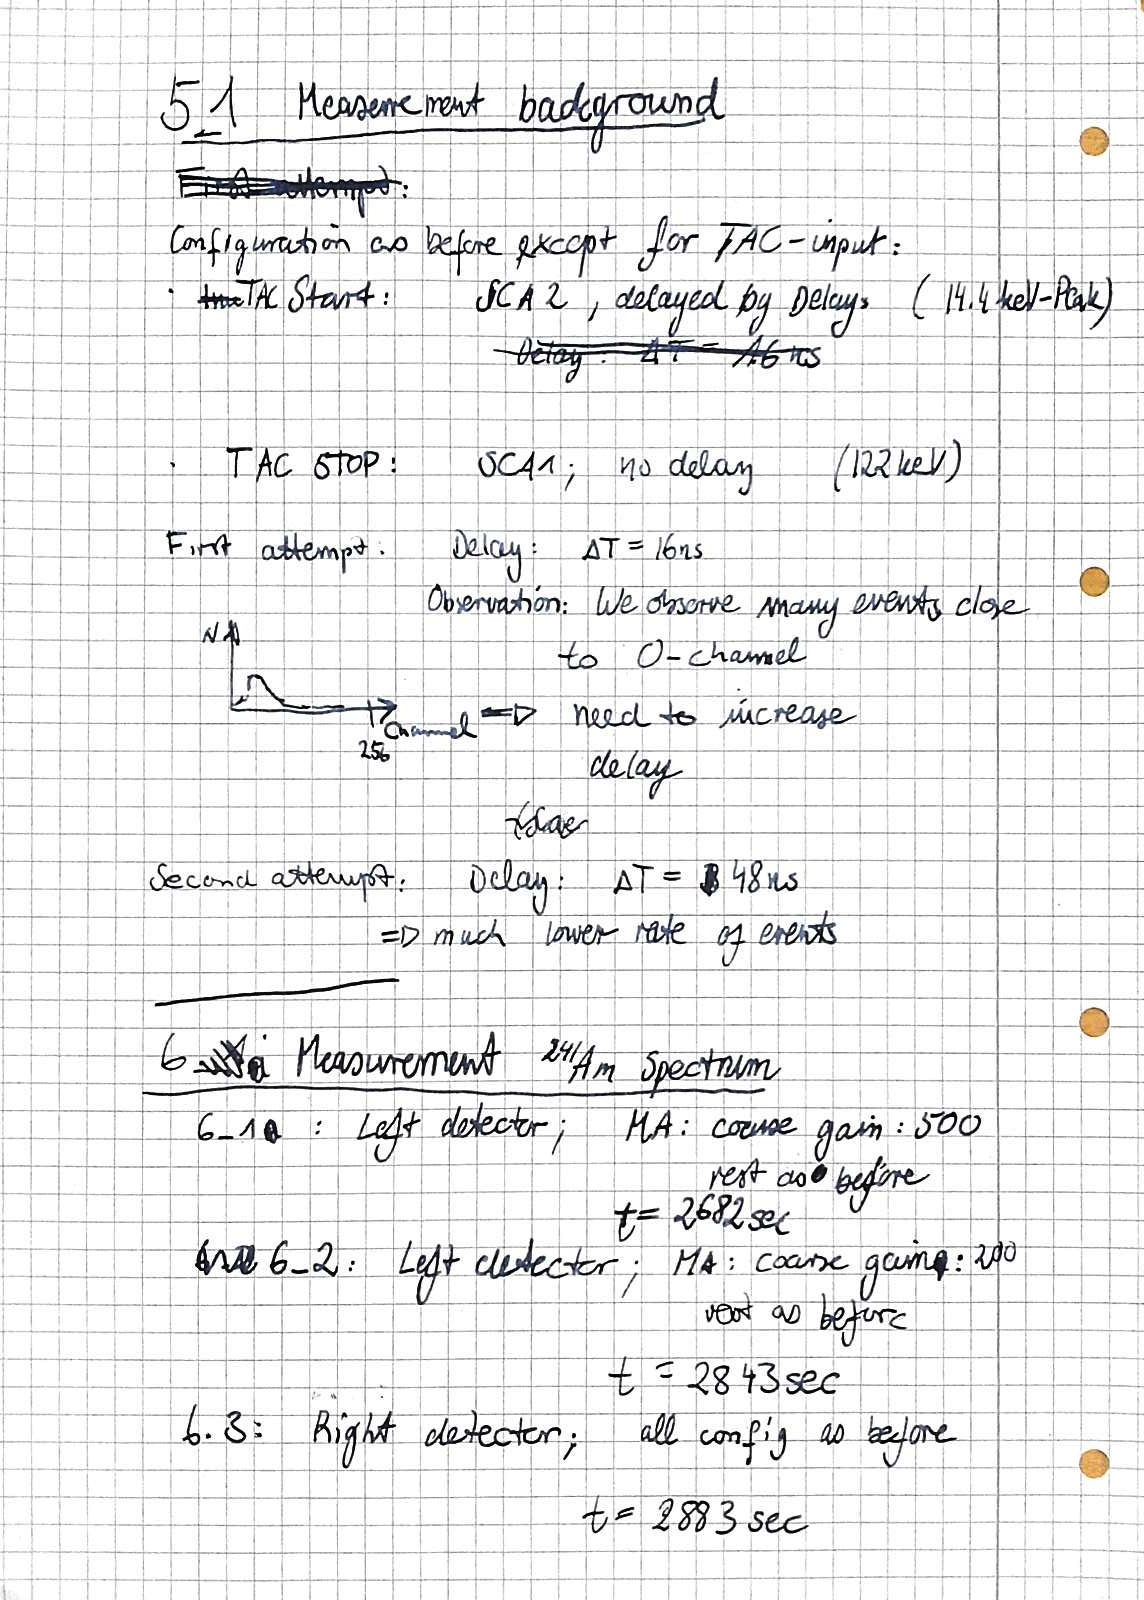
\includegraphics[width=\linewidth]{records/page8.jpeg}
    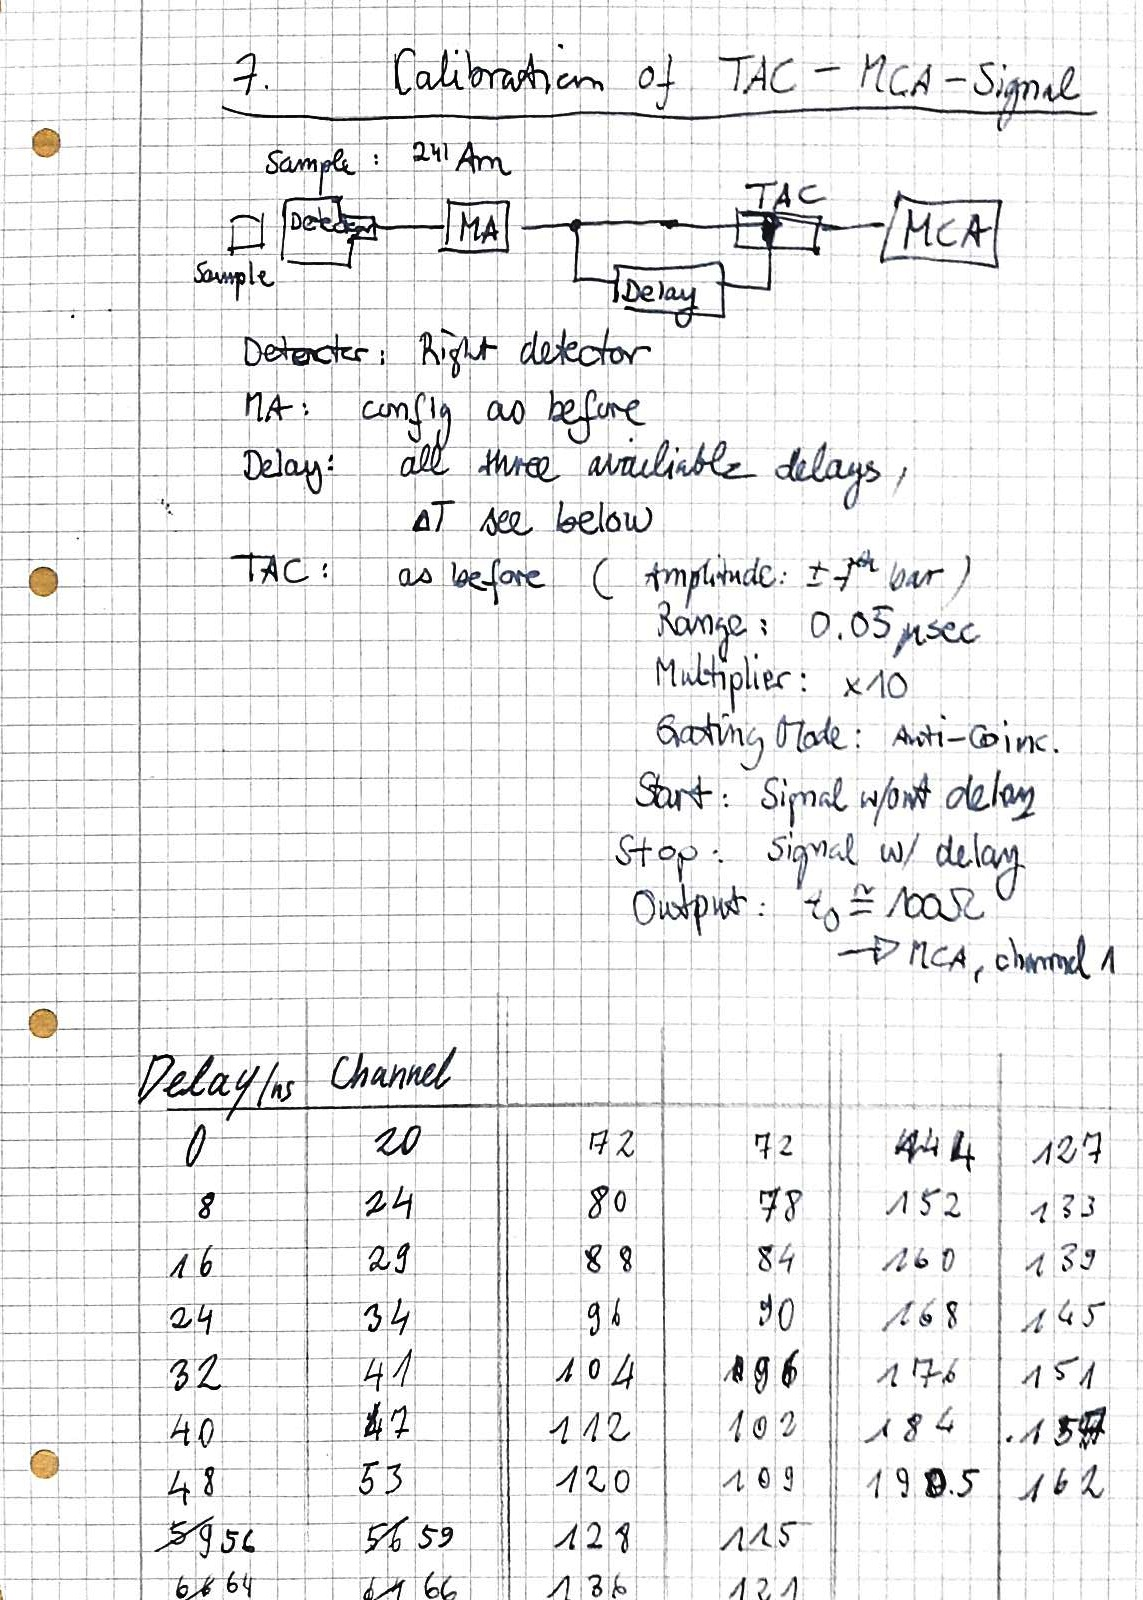
\includegraphics[width=\linewidth]{records/page9.jpeg}
    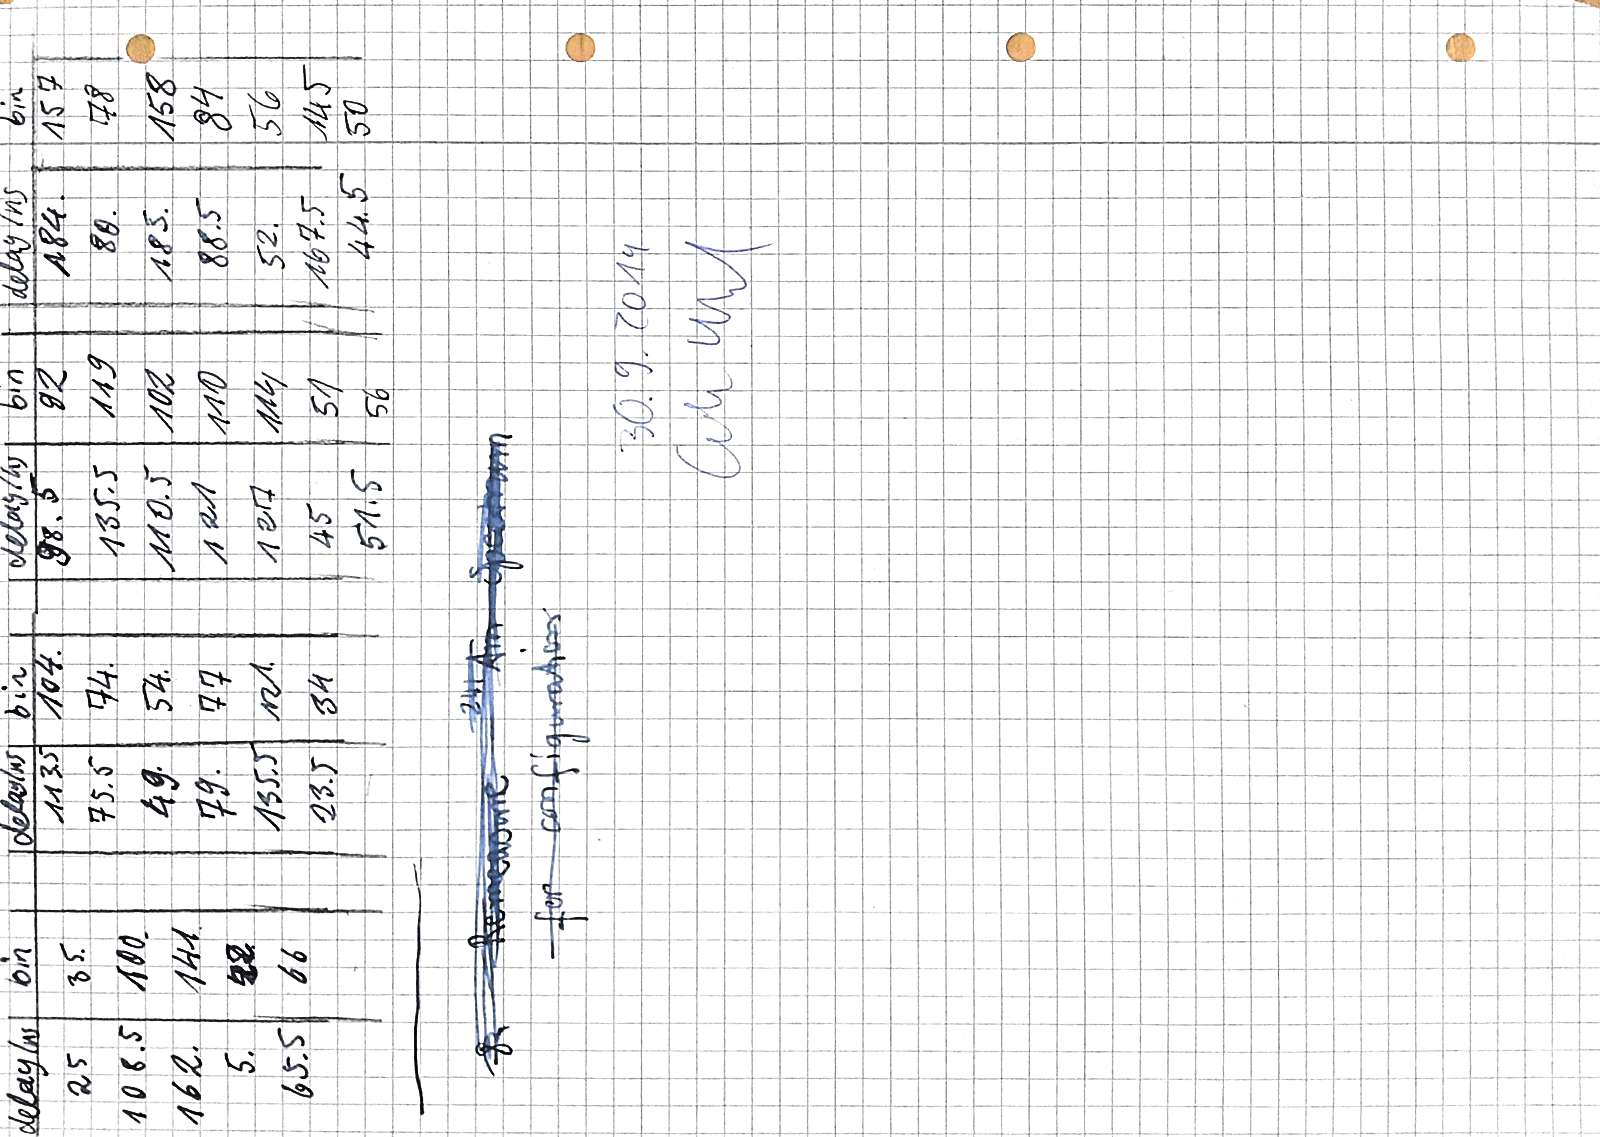
\includegraphics[width=\linewidth]{records/page10.jpeg}
\clearpage

